\documentclass[11pt]{article}
\usepackage[T1]{fontenc}
\usepackage{lmodern}
\usepackage[margin=1in]{geometry}
\usepackage{amsmath,amssymb,amsthm}
\usepackage{booktabs,tabularx,array,longtable}
\usepackage{placeins}
\usepackage{microtype}
\usepackage[table]{xcolor}
\usepackage{listings}
\usepackage{tikz}
\usetikzlibrary{arrows.meta,positioning}
\usepackage[obeyspaces,spaces]{url}
\usepackage[colorlinks=true,linkcolor=blue!45!black,citecolor=blue!45!black,
  urlcolor=blue!45!black]{hyperref}
\hypersetup{
  pdftitle={Gaussian Quadrature in Lean and Rocq},
  pdfauthor={Robert Joseph}}
\definecolor{provedcolor}{HTML}{126447}
\definecolor{partialcolor}{HTML}{875000}
\definecolor{opencolor}{HTML}{435B77}
\definecolor{refutedcolor}{HTML}{A12935}
\definecolor{tablehead}{HTML}{EDF2F5}
\definecolor{codebackground}{HTML}{F5F7F8}
\lstdefinestyle{papercode}{
  basicstyle=\small\ttfamily,
  keywordstyle=\color{blue!50!black}\bfseries,
  commentstyle=\color{provedcolor},
  stringstyle=\color{partialcolor},
  backgroundcolor=\color{codebackground},
  frame=single,rulecolor=\color{opencolor!30},
  framerule=0.4pt,framesep=7pt,
  xleftmargin=8pt,xrightmargin=8pt,
  columns=fullflexible,keepspaces=true,
  showstringspaces=false,upquote=true,
  breaklines=true,captionpos=b,
  aboveskip=12pt,belowskip=12pt
}
\lstdefinelanguage{Lean}{
  morekeywords={def,theorem,by,have,exact,unfold,rw,linarith,cas},
  morecomment=[l]{--},
  literate={ℝ}{{\ensuremath{\mathbb{R}}}}1
           {∫}{{\ensuremath{\int}}}1
           {≤}{{\ensuremath{\le}}}1
           {·}{{\ensuremath{\cdot}}}1
}
\lstset{style=papercode}
\newcommand{\halfcircle}{%
  \tikz[baseline=-0.3ex,x=1ex,y=1ex]{%
    \fill (0,0) -- (0,0.6) arc[start angle=90,end angle=270,radius=0.6] -- cycle;
    \draw[line width=0.5pt] (0,0) circle[radius=0.6];}}
\newcommand{\checked}[1]{\textcolor{provedcolor}{\ensuremath{\checkmark}\,\textbf{#1}}}
\newcommand{\proved}{\checked{Proved}}
\newcommand{\partialproof}{\textcolor{partialcolor}{\halfcircle\,\textbf{Partial}}}
\newcommand{\conditional}{\textcolor{partialcolor}{\halfcircle\,\textbf{Conditional}}}
\newcommand{\openproof}{\textcolor{opencolor}{\ensuremath{\circ}\,\textbf{Open}}}
\newcommand{\refuted}{\textcolor{refutedcolor}{\ensuremath{\times}\,\textbf{Refuted}}}
\newtheorem{theorem}{Theorem}[section]
\newtheorem{proposition}[theorem]{Proposition}
\newcommand{\R}{\mathbb{R}}
\newcommand{\fl}{\operatorname{fl}}
\newcommand{\real}{\operatorname{real}}
\newcommand{\I}{\mathcal{I}}
\newcommand{\Q}{\mathcal{Q}}
\newcommand{\code}[1]{%
  \ifmmode\text{\texttt{\detokenize{#1}}}\else\nolinkurl{#1}\fi}
\newcolumntype{Y}{>{\raggedright\arraybackslash}X}
\title{Gaussian Quadrature in Lean and Rocq}
\author{Robert Joseph\\[0.3em]
  \normalsize California Institute of Technology}
\date{}

\begin{document}
\maketitle

\begin{abstract}
We formalize Gaussian quadrature in Lean, starting from Appel and Bindel's
preliminary Rocq development and comparing the proofs needed to connect real analysis,
floating-point arithmetic, and C execution. Using mathlib, LeanPDE, and
FloatLib, we construct weighted Gaussian rules of every positive order on
compact intervals, prove their remainder and convergence, and certify
binary64 results for all ten rules stored in the example program. Checking
the example exposes two incorrect error bounds: $0.00223$ for two nodes
and $0.02$ for one node. We prove the replacements $0.00356$ and $0.159$,
correct the remainder's inconsistent node indexing, model the weight
actually stored in C, and give counterexamples
to three admitted helper lemmas. For the C proof, we replace the external
cosine with a verified polynomial. For each stored rule, every permitted
evaluation order of an initialized call then terminates with the certified
result in our Lean adaptation of CompCert's C semantics. We prove that
translation to Clight preserves these calls, and that the C return values
agree with the result annotations of ten assembly applications verified
directly in Lean. Independent Rocq proofs use CompCert's compiler theorem.
The Lean result concerns these particular programs; general correctness of
source translation and compilation, and agreement between the Lean and Rocq
definitions of execution, remain open.
\end{abstract}

\section{Introduction}
\label{sec:intro}

Appel and Bindel~\cite{appelbindel} study the verification of a C program
that approximates
\begin{equation}
  \I(f)=\int_{-1}^{1}f(x)\,dx,
  \qquad f(x)=\tfrac12(1-x)\cos x,
  \label{eq:example}
\end{equation}
using Gaussian quadrature. The integrator occupies seven lines of C. Yet
proving its accuracy requires real analysis, floating-point error bounds,
memory and function-call reasoning, and a theorem about compilation. This
makes it a useful example for comparing Lean and Rocq: the program is small
enough to inspect, while its correctness depends on all of these proofs.

Their paper is titled \emph{Formalization of Gaussian Quadrature and
Application Verification (Preliminary Draft)}. Its admitted lemmas mark
unfinished work. We review that preliminary version and the accompanying
public source, distinguishing false statements from missing proofs and
unassembled program modules. The source already contains work on correcting
the derivative-bound hypotheses; we discuss its status in
Section~\ref{sec:admitted}. Our results are in a separate development and
do not complete the authors' Rocq files.

Their Rocq development brings together MathComp and
MathComp-Analysis~\cite{mathcomp,mathcompanalysis} for real analysis,
Flocq~\cite{flocq} for floating-point arithmetic, LAProof~\cite{laproof}
for rounding error in sums, Interval~\cite{interval} for concrete
inequalities, and VST~\cite{vstfloyd} for C verification. CompCert's
compiler theorem~\cite{compcert} provides the next connection, from
verified source behavior to formal assembly. Our development,
LeanQuadrature, uses mathlib~\cite{mathlib}, LeanPDE~\cite{leanpde}, and
FloatLib~\cite{floatlib} for the mathematical and numerical proofs. For
execution, we adapt CLean~\cite{clean} and prove the required properties
directly from the language semantics.

The example also lets us check its accuracy claims independently of the
program proof. The integral is $\sin1$, and the exact two-point rule
returns $\cos(1/\sqrt3)$. Their difference is about $0.0035591571$, which
already exceeds the manuscript's bound of $0.00223$. The one-point bound
is also false. We prove corrected bounds, identify inconsistent indexing
in the admitted remainder theorem, and use the actual C weight where the
original floating-point model differs. Section~\ref{sec:discrepancies}
gives the calculations and counterexamples. It also distinguishes three
false admitted helper lemmas from unfinished program obligations, such as
the missing callback body proof and module assembly. An admitted lemma is an assumption:
checking a proof that uses it does not establish that assumption.

Our mathematical results apply beyond this integrand. For every positive
order, we construct a Gaussian rule on a compact interval with a positive
continuous weight. We prove exactness, positivity of the weights, the
three-term recurrence, the integrated remainder, and convergence for
continuous integrands. The original development supplies concrete root
certificates through four nodes and leaves the general remainder admitted.
Our floating-point results cover all ten rules stored in its C source,
with error bounds for the actual constants and rounded operations.
Appendix~\ref{sec:stewart-map} maps all 24 numbered paragraphs of their
mathematical presentation to the results available in LeanPDE and identifies
the declarations used by LeanQuadrature.

At the C level, we replace the external cosine with a polynomial whose C
body and numerical use are both verified. We prove that initialized calls
to the integrator terminate with the certified result in every evaluation
order permitted by our adapted semantics. We then prove that the six
selected library functions preserve their call results when translated to
Clight, CompCert's simpler intermediate language for C. The application
programs report the same binary64 values and exit zero; we prove this
behavior through formal assembly in Lean. We also prove those application
results independently in Rocq, where they compose with CompCert's compiler
theorem.

The C library and assembly applications expose their results differently.
A library call returns a value without producing an event. The application
records that value in a semantic annotation, then exits. We prove that these
observations agree for all ten orders, including the original two-point
wrapper. This connects the results of the particular programs. It does not
prove that compiling the original C text produces the imported assembly
trees. General source-translation and compiler correctness, and agreement
between the adapted Lean and Rocq execution rules, remain open.

\subsection{The five levels of verification}
\label{sec:levels}

The five levels are the real integral, the exact quadrature rule, its
floating-point model, the C implementation, and the compiled program.
Four proofs connect adjacent levels. Write $\Q_n(f)$ for the exact
quadrature sum and $F$ for the binary64 result of the rounded functional
model. The first two connections establish
\begin{equation}
 |\I(f)-\Q_n(f)|\le E_{\mathrm{quad}},
 \qquad
 |\Q_n(f)-\real(F)|\le E_{\mathrm{fp}}.
 \label{eq:two-errors}
\end{equation}
The first inequality bounds quadrature error over the reals. The second
accounts for stored constants, callback error, and rounding. The triangle
inequality then gives
\[
  |\I(f)-\real(F)|\le E_{\mathrm{quad}}+E_{\mathrm{fp}}.
\]
The third proof shows that the C function returns $F$, with valid memory
accesses and calls. The fourth preserves that source behavior through
compilation. These last two proofs introduce no new numerical error; their
task is to preserve the computation already analyzed.

The cosine implementation affects what can be concluded at the C level.
The original program calls an external cosine, so its verification needs a
contract for that implementation. Our replacement polynomial has a verified
C body and certified numerical results at the inputs used by the example.
We also prove initialization of the stored tables. The resulting library
theorems therefore need neither an assumed cosine contract nor an assumed
table predicate.

Table~\ref{tab:comparison} compares this work with Appel and Bindel's
development. The independent Rocq application proofs that we use with
CompCert are described separately in Section~\ref{sec:compilation}; they
are part of LeanQuadrature, not changes to the authors' Rocq proofs.

\medskip
\noindent
\fcolorbox{opencolor!25}{tablehead}{%
\begin{minipage}{\dimexpr\textwidth-2\fboxsep-2\fboxrule\relax}
\small
\textbf{Reading the labels.}\quad
\proved{} means the stated theorem is checked under its hypotheses.
\partialproof{} and \conditional{} mean an application still has
obligations to discharge. \openproof{} means the connection is not proved.
\refuted{} means a counterexample disproves the claim.
\end{minipage}}

\begin{table}[htbp]
\centering
\small
\renewcommand{\arraystretch}{1.12}
\begin{tabularx}{\textwidth}{@{}>{\raggedright\arraybackslash}p{2.1cm}YY@{}}
\toprule
\rowcolor{tablehead}
Level & Appel--Bindel in Rocq & LeanQuadrature in Lean\\
\midrule
1. Real integral &
\textbf{MathComp, MathComp-Analysis}: weighted real integral. &
\textbf{mathlib}: interval integrals.
\textbf{LeanPDE}: checked symbolic integration.
\proved{}: the example integral equals $\sin1$.\\
\addlinespace
2. Numerical rule &
\textbf{MathComp, MathComp-Analysis}.
\partialproof{}: recurrence and quadrature proofs, with root certificates
through four points. The general remainder is admitted; convergence is
unproved. &
\textbf{mathlib, LeanPDE}: the shared Gaussian theory.
\proved{}: construction at every positive order on compact intervals;
exactness, positive weights, recurrence, the corrected remainder,
and convergence.\\
\addlinespace
3. Rounded model &
\textbf{Flocq, LAProof, Interval}.
\partialproof{}: rounded fold and error analysis.
The example's accuracy argument uses admitted numerical helpers;
two overflow helpers have false conclusions for permitted parameters. &
\textbf{FloatLib}: binary64 arithmetic and rounding bounds.
\textbf{LeanPDE}: root and weight enclosures.
\proved{}: finite fold, error bounds, and ten stored rules;
callback accuracy at the inputs used by the examples.\\
\addlinespace
4. C execution &
\textbf{VST}.
\checked{Body proof}: VST relates the integrator to its functional model under
table and callback specifications.
\partialproof{}: the wrapper uses admitted numerical lemmas;
the callback body and assembly into a Verified Software Unit (VSU),
including global initialization, remain obligations. &
\textbf{Adapted CLean, FloatLib}, with our execution proofs.
\proved{}: initialized calls using the original functions and a verified
C cosine polynomial, at ten orders and in every permitted evaluation order.
Behavioral preservation to Clight for all six selected functions.
\openproof{}: general source-translation correctness and agreement
with Rocq's execution semantics.
The external-cosine variant retains its contract.\\
\addlinespace
5. Compilation &
\textbf{CompCert}.
\checked{Compiler theorem}: CompCert preserves program behavior.
Using it for this application requires source correctness in its C semantics. &
\textbf{Adapted CLean}, with our assembly proofs.
\checked{Particular programs}: direct proofs for ten polynomial applications
at formal assembly, reporting the values returned by the C library.
\openproof{}: a verified compiler, or a transfer of CompCert's theorem into Lean.\\
\bottomrule
\end{tabularx}
\caption{Libraries and proof coverage at each level. The Rocq column describes
Appel and Bindel's preliminary development, including the admitted dependencies discussed in
Section~\ref{sec:discrepancies}. Our C proofs use a verified polynomial in
place of the external cosine. Their return values agree with the assembly
applications' result annotations by Theorem~\ref{thm:c-assembly-observations}.
That theorem concerns these programs' behavior, not the correctness of a
general compiler.}
\label{tab:comparison}
\end{table}

LeanPDE supplies the weighted Gaussian theory, explicit Legendre rules
through four nodes, and general root and weight certificate proofs.
These results build on mathlib and LeanPDE's quadrature interfaces,
midpoint rule, and two-point rule.
Rational interval arithmetic, Taylor bounds, and integration tactics provide concrete
enclosures. Its sharp two-point error bound, proved with a Peano kernel,
and its general Hermite remainder give two proofs of the fourth-derivative
bound for that rule.
LeanQuadrature contains the stored tables, their particular root brackets,
numerical accuracy certificates, and program proofs. FloatLib supplies
the binary64 operations and rounding theorems.

\section{Corrections to the example and its proofs}
\label{sec:discrepancies}

Both the integral and the ideal quadrature sum have closed forms, so we
can check the claimed errors directly. A quartic tests the remainder
formula, and decoding the table literals tests whether C and the rounded
model store the same values. Table~\ref{tab:corrections} records these four
findings. The rest of this section examines the admitted helpers and
program specifications on which the application proof depends.
These are corrections to a preliminary development. The absence of a proof
is a coverage question; a counterexample establishes the stronger claim
that a statement must change before it can be proved.
Page references and source claims concern the examined preliminary manuscript
and accompanying source~\cite{appelbindel,appelbindelcode}; the repository
records their exact versions and maps each finding to its declarations.

\begin{table}[htbp]
\centering
\small
\renewcommand{\arraystretch}{1.15}
\begin{tabularx}{\textwidth}{@{}>{\raggedright\arraybackslash}p{2cm}YY@{}}
\toprule
\rowcolor{tablehead}
Location & Finding & Correction checked in Lean\\
\midrule
Page 5, two points &
\refuted{}: the ideal error bound $0.00223$. &
\proved{}: the replacement bound $0.00356$.
Actual error $\approx0.0035591571$.\\
\addlinespace
Page 5, one point &
\refuted{}: the ideal error bound $0.02$. &
\proved{}: the replacement bound $0.159$.
Actual error $1-\sin1\approx0.1585290152$.\\
\addlinespace
Page 4, remainder &
\refuted{}: the formula combines $n$ nodes with a derivative of order
$2n+2$ and the polynomial $p_{n+1}$. &
\proved{}: the remainder uses $2n$ derivatives and $p_n$,
with $C^{2n}$ regularity. Two nodes require the fourth derivative.\\
\addlinespace
Pages 6--7, weight &
\checked{Mismatch proved}: the C and model weights have different binary64
bits; the C value exceeds the stated tolerance. &
\proved{}: the C value satisfies a $5\cdot10^{-16}$ weight bound.
Our initialized library uses these actual C bits.\\
\bottomrule
\end{tabularx}
\caption{Corrections and their proof status. The first three rows concern
real mathematics. The fourth repairs the numerical model to match the
stored C constant and uses it in the initialized Lean library.}
\label{tab:corrections}
\end{table}

\subsection{The two-point error bound}

Page 5 states the bound $223/100000=0.00223$ for the exact-real two-point
rule. Symmetry in~\eqref{eq:example} gives
\[
 |\I(f)-\Q_2(f)|
  =|\sin1-\cos(1/\sqrt3)|
  \approx0.0035591571.
\]
The error is larger than the proposed bound. The Lean proof works with rational
enclosures for sine and cosine, so the displayed decimal is only an
illustration. An upper enclosure for $\sin1$ and a lower enclosure for
$\cos(1/\sqrt3)$ also give the corrected bound $0.00356$.
Listing~\ref{lst:lean-bound} shows the final proof. The first rewrite
replaces the integral and the sum by their closed forms, and the two
remaining goals are linear inequalities between previously proved
enclosures.

\begin{lstlisting}[language=Lean,float=htbp,
  caption={The corrected two-point bound, from \code{Quadrature.Examples.TwoPointCosine}.
  The enclosure lemmas are proved earlier in the same module.},
  label={lst:lean-bound}]
theorem corrected_two_point_bound :
    |(∫ x in (-1 : ℝ)..1, integrand x) -
      (integrand (-(1 / Real.sqrt 3)) + integrand (1 / Real.sqrt 3))| ≤
      (356 / 100000 : ℝ) := by
  rw [integral_eq, two_point_eq, abs_of_nonneg]
  · linarith [sin_one_upper, cos_node_lower]
  · linarith [sin_one_lower, cos_node_upper]
\end{lstlisting}

The C corollary on pages 1 and 11 uses the slightly larger bound $0.00224$
for the reported result \code{0.83791182769499317}. Its analytic premise
therefore needs correction before the program argument can establish an
accuracy bound. The counterexample above concerns the ideal rule. To prove
an error bound for a C execution, we must also account for its cosine
implementation and rounded operations, as in
Sections~\ref{sec:floating} and~\ref{sec:programs}.

\subsection{The one-point error bound}

The one-point node is zero and its weight is two, so
\[
  \Q_1(f)=2f(0)=1,\qquad
  |\I(f)-\Q_1(f)|=1-\sin1\approx0.1585290152.
\]
This exceeds the bound $2/100=0.02$ on page 5 by almost a factor of eight. We
prove both the failure of that inequality and the replacement bound
$159/1000=0.159$ in Lean.

\subsection{Counting nodes and derivatives}

The displayed \code{quadrature_error} statement on page 4 uses an $n$-node
root collection together with a derivative of order $2n+2$ and a polynomial
indexed by $n+1$. With $n$ the number of nodes, the remainder requires
order $2n$, as in Theorem~\ref{thm:remainder}. The source makes the node
count explicit: its root certificate stores an $n$-tuple, and the
quadrature sum ranges over $i<n$.

The formula $2n+2$ is right for a rule with $n+1$ nodes indexed from zero
through $n$, which is Stewart's convention~\cite{stewart}. The problem is
that the node count and the derivative order follow different conventions
in the same statement. For two nodes the required derivative is the
\emph{fourth}, and for one node it is the second.

A quartic makes the consequence concrete. For $f(x)=x^4$, two-point
quadrature has error
\[
 \int_{-1}^{1}x^4\,dx
   -\left[(-1/\sqrt3)^4+(1/\sqrt3)^4\right]
   =\frac25-\frac29=\frac8{45},
\]
while $f^{(6)}$ is identically zero. The displayed formula would give zero
error. Lean proves the exact error $8/45$ and the vanishing sixth
derivative, which together refute that formula for a two-node rule.

The manuscript marks the general remainder theorem as admitted. Its source
statement also quantifies over an arbitrary \code{f : R -> R} with no
smoothness premise. Our theorem, \code{GaussianRule.remainder}, uses the
derivative of order $2n$ and requires $C^{2n}$ regularity on the closed
interval. Section~\ref{sec:mathematics} explains the proof.

\subsection{A weight differs between C and the model}

The C listing on page 6 stores the outer three-point weight as
\code{0.555555555555556}. The functional-model value on page 7 is
\code{0.5555555555555556}. In binary64 these are different numbers:
\begin{center}
\begin{tabular}{ll}
\toprule
C literal & \code{0x3fe1c71c71c71c76}\\
Functional-model literal & \code{0x3fe1c71c71c71c72}\\
\bottomrule
\end{tabular}
\end{center}
The C value decodes exactly to $2501999792983611/4503599627370496$. Its
distance from the ideal weight $5/9$ is
\[
  \frac{19}{40532396646334464}
      \approx4.6876083262\cdot10^{-16},
\]
which exceeds $2^{-53}$. So the C constant misses the stated uniform
half-ulp tolerance even when half an ulp is measured at one. Lean proves
this inequality and the difference between the two stored values. We keep
the original C constant and prove the uniform weight bound $5\cdot10^{-16}$
for the stored tables instead.

The mismatch also affects the program proof. The generated Clight program
contains the C bits, but the table predicate in the VST specifications
describes the model's array. A body theorem may assume that predicate, but
a proof from program initialization must establish it for the array that is
actually there, and with these literals it cannot. We model the existing C
literals and enlarge the error budget. Our selected library
initializes those values and proves the required table predicate. The
original VST development would need a corresponding change to its model
and initialization proof. VST's Verified Software Unit construction checks
the connection between global initializers and the module's data predicate.
The quadrature source has not yet assembled this VSU, so the successful
body proofs do not assert that initialization satisfies their table
premise~\cite{vstvsu}.
The middle three-point weight has different decimal spellings in the two
files, but both spellings round to the same binary64 value, so that entry
is not a second mismatch.

\subsection{Assumptions in the original proofs}
\label{sec:admitted}

The two example lemmas, \code{error_1_0_1} and \code{error_1_0_2}, use
\code{quadrature_error_bound_is_bound}, which depends on a Legendre
specialization of the admitted \code{quadrature_error}. Interval checks an
inequality derived from the assumed remainder. The remainder itself
remains an assumption, so a later proof ending in \code{Qed} establishes
an implication from that assumption. This explains how the final scripts
can compile while the claimed error bound is false: the unchecked premise
already contains the error.

The C development has a similar dependency. Its integrator body proof is complete
under its specification. The example wrapper invokes admitted lemmas for
function bounds, derivative bounds, callback accuracy, and quadrature
error. The verification file supplies nine body lemmas for ten internal
functions and never proves \code{body_testfun}. The wrapper obtains the
callback contract from the global specification environment with
\code{make_func_ptr}, which establishes what may be assumed about the
callback, not that its C body meets the contract.

To see exactly what the completed proofs depend on, we rebuilt the original
quadrature proofs and their LAProof dependencies and asked Rocq for the
transitive assumptions of 43 declarations. The wrapper depends on ten of
the twelve admitted declarations in the quadrature files, including the
false positivity and overflow helpers described below. The integrator body
depends on none of the twelve. The rebuild needed two explicit product-type
annotations in the high-level 2D specifications, which resolve a notation
ambiguity in our Rocq environment and change no proof, admitted lemma, or C
code. All nine original body proofs then compile. The committed Clight
syntax was generated for AArch64 with the Apple ABI, and our review checks
it under an x86-64 CompCert configuration.

The preliminary manuscript acknowledges the missing remainder proof.
Consequently its concluding description of a first-principles argument
should be read as the intended completed chain. The checked state of that
chain still includes the assumptions above.

\paragraph{Work already under way on derivative bounds.}
The public source includes a separate \code{proof/g_max_deriv.v} that
reformulates \code{fbound} and \code{deriv_bound} on a fixed interval with
$a<b$. It requires both the starting and perturbed arguments to lie in
that interval. Its target bounds the change in the function by a derivative
bound times the displacement. This is the appropriate mean-value argument
for controlling perturbed quadrature nodes.
The file is work in progress: \code{g_max_deriv} ends in \code{Qed} but
uses the admitted \code{g_max_deriv_oneway}, and other admissions remain.
It is separate from the integrated quadrature proofs in the examined
revision~\cite{appelbindelcode}. This ongoing correction is relevant to the
example's admitted function and derivative bounds. Our accuracy theorem
states the required Lipschitz bound explicitly, and the concrete numerical
certificates establish their own bounds.

\paragraph{A positive function with zero integral.}
The admitted lemma \code{Rintegral_gt_0} assumes continuity,
nonnegativity, and a nonzero value somewhere in $[a,b]$, and concludes
that the integral is positive. The missing condition is $a<b$. For $a=b=0$
and $h(x)=1$, all three premises hold, but
\[
  \int_{[0,0]}h(x)\,dx=0
\]
because a singleton has Lebesgue measure zero. Our Lean counterexample
checks the three premises and refutes the conclusion. We also check the
example in Rocq with MathComp-Analysis, and a separate diagnostic applies
the original admitted lemma to those premises and derives a contradiction.
The source uses this helper in its polynomial-positivity argument, inside a
section that already assumes $a<b$, so adding the missing premise is a
natural repair for that use. Our \code{polynomialIntegral_square_pos}
requires $a<b$ and proves the result using mathlib.

\paragraph{A specification that names the wrong function.}
The source also includes Hughes quadrature routines for a triangle. Its
\code{hughes_weight_spec} begins with \code{DECLARE _gauss2d_weight}
where the intended identifier is \code{_hughes_weight}. As a result,
\code{quadrules_ASI} contains two specifications named
\code{_gauss2d_weight} and none named \code{_hughes_weight}. The body proof
still checks because VST's \code{semax_body} receives a function body and
an identifier--contract pair, checks the body against the contract, and
discards the identifier. Associating names, bodies, and contracts is a
separate obligation when the verified interface is assembled. A VSU checks
that the specification used at a call is supplied by the corresponding
body or by a contract that implies it~\cite{vstvsu}. That is the missing
integration step here. The identifier can be corrected
without changing the contract, and the existing body theorem then proves
the retagged specification. This is a defect in the specification of the
triangle routine, not a counterexample to its numerical result.

\subsection{Two overflow lemmas need stronger hypotheses}
\label{sec:overflow}

The floating-point proof must show that every intermediate result is
finite. The source introduces a condition named \code{parameter_limits}
and leaves two helper inequalities admitted. Neither helper follows from
the stated conditions for all permitted parameters, and the problem can be
seen without running any floating-point code.

Specialize to binary64 and write
\[
  u=2^{-53},\qquad \eta=2^{-1075},\qquad T=2^{1024}.
\]
These are the relative-error constant, the absolute-error constant, and
\code{fmax} in the version of LAProof used by the source.
The largest finite binary64 number is smaller than $T$.
Take one node, the zero
integrand, and a callback that always returns zero. Choose the valid but
loose function bound $F=T/4$ and set the derivative and callback-error
bounds to zero. The node zero and the weight two are represented exactly.
The source's range condition becomes
\[
  \left(1+\frac{u}{1+u}\right)(2+u)\frac{T}{4}+\eta<T,
\]
which holds, and its earlier product helper also holds. But the admitted
\code{finite_integrate_model_aux} would require
\begin{equation}
  \frac{T}{2}+\frac{T}{4}(u^2+3u)+\eta
       <\frac{T}{2(1+u)}.
  \label{eq:overflow-counterexample}
\end{equation}
The left side is greater than $T/2$ and the right side is smaller. This is
a counterexample at a positive order, with valid bounds for both the
mathematical function and the callback.

The other helper, \code{gauss_pt_wt_limit_aux}, fails at zero nodes, which
the source's type \code{'I_5} permits. With function bound $F=T$ and zero
callback error, \code{parameter_limits} reduces to $0<T$, while the helper
requires $2T(1+u)+\eta<T$. Either the empty reduction needs separate
treatment or the helper needs a positive-order premise.

Lean checks both counterexamples in \code{Quadrature.Examples.Overflow}
with exact arithmetic on the transcribed inequalities. Both callbacks
return zero, and their actual computations stay finite. The contradictions
concern the proposed sufficient conditions for the helper lemmas.
LAProof's summation theorem has its own valid precondition; the missing
step is to derive it inside the quadrature development. Our finiteness
proof, in Section~\ref{sec:floating}, bounds the sum of absolute products
together with the accumulated rounding errors.

\section{Gaussian rules in Lean}
\label{sec:mathematics}

The remainder theorem depends on the nodes, weights, and polynomial
exactness of the rule.
Appel and Bindel follow Stewart~\cite{stewart}: they construct the monic
orthogonal polynomials by the three-term recurrence and take a
\code{roots_of_ortho_p n} certificate containing $n$ ordered roots, which
their concrete Legendre instances supply through four points. We construct
the orthogonal polynomials by orthogonal projection, prove the existence
of their roots by factorization and integral positivity, and derive the
recurrence afterward.
This yields a Gaussian rule for every positive order. The construction
uses mathlib's polynomial algebra, orthogonal projection in
finite-dimensional inner product spaces, and Lagrange interpolation. Its
remainder and convergence proofs use Rolle's theorem and uniform
polynomial approximation. LeanPDE provides this general theory and the
concrete Legendre rules. Appendix~\ref{sec:stewart-map} maps the mathematical
paragraphs to its definitions and theorems.

Fix $a<b$ and a continuous function $w:[a,b]\to\R$ with $w(x)>0$. The
intended integral is
\[
  \I_w(f)=\int_a^b f(x)w(x)\,dx.
\]
For a positive integer $n$, a Gaussian rule consists of distinct interior
nodes $x_i$ and weights $\lambda_i$, with
$\Q_n(f)=\sum_{i=1}^n\lambda_i f(x_i)$. Throughout the paper $n$ is the
\emph{number of nodes}.

\subsection{Choosing the nodes and weights}

The integral defines an inner product on real polynomials,
$\langle p,q\rangle=\I_w(pq)$. It is positive definite because a nonzero
polynomial cannot vanish on a nondegenerate interval, so its square has
positive integral against $w$. Orthogonal projection onto the polynomials
of degree less than $n$ constructs the unique monic polynomial $p_n$ of
degree $n$ orthogonal to that space.

The root argument shows that $p_n$ has exactly $n$ distinct roots in
$(a,b)$, and these are the nodes. Lagrange interpolation defines the
weights. Polynomial division by $p_n$ then proves exactness:
\begin{equation}
  \Q_n(q)=\I_w(q)
  \quad\text{whenever}\quad \deg q\le 2n-1.
  \label{eq:exactness}
\end{equation}
Writing $q=p_ns+r$ gives $\deg s<n$ and $\deg r<n$. Orthogonality kills the
integral of $p_ns$, and evaluation at the nodes kills its quadrature sum.

If $\ell_i$ is the $i$th Lagrange basis polynomial, exactness applies to
$\ell_i^2$ and gives $\lambda_i=\I_w(\ell_i^2)>0$. Applying exactness to
the constant polynomial gives $\sum_i\lambda_i=\I_w(1)$. These two facts
control perturbations of the integrand later without estimating each
weight separately. The development also proves the three-term recurrence,
including the positivity of the norm ratio, and identifies the explicitly
represented low-order Legendre rules with the constructed monic family.

\subsection{Integrating the remainder}

\begin{theorem}[Integrated Gaussian remainder]
\label{thm:remainder}
Let $a<b$, let $w$ be positive and continuous on $[a,b]$, let $n>0$, and let
$f\in C^{2n}([a,b])$. For the Gaussian rule constructed above, there exists
$\xi\in[a,b]$ such that
\begin{equation}
 \I_w(f)-\Q_n(f)
  = \frac{f^{(2n)}(\xi)}{(2n)!}\int_a^b p_n(x)^2w(x)\,dx .
 \label{eq:remainder}
\end{equation}
\end{theorem}

In Lean the smoothness hypothesis is \code{ContDiffOn} on the closed
interval, and the derivative is the iterated derivative within that
interval, so we never assume a smooth extension beyond the integration
domain. More precisely, the proof takes functions $F_0,\ldots,F_{2n}$
continuous on $[a,b]$, with $F_k'=F_{k+1}$ on $(a,b)$ for $k<2n$.
The \code{ContDiffOn} version supplies this chain using
\code{iteratedDerivWithin}.

Taylor--Lagrange itself is already in the mathlib revision used here:
\code{taylor_mean_remainder_lagrange} gives the Taylor remainder about one
center. Our added interpolation theorem concerns $n$ distinct nodes,
matching the function and its first derivative at each node. It is this
Hermite remainder, followed by an integral argument, that proves
Theorem~\ref{thm:remainder}. We do not formalize arbitrary prescribed
derivative multiplicities in the interpolant.

Let $H$ be the Hermite interpolant of degree below $2n$ matching both $f$
and $f'$ at the nodes. For a point $x$ that is not a node, choose
$c=(f(x)-H(x))/p_n(x)^2$ and consider
\[
  G(y)=f(y)-H(y)-c\,p_n(y)^2.
\]
There are double zeros at the $n$ nodes and one more zero at $x$. Repeated
Rolle supplies a zero of the $2n$th derivative. Since $H^{(2n)}=0$ and
$(p_n^2)^{(2n)}=(2n)!$, this identifies $c$. At a node the pointwise
remainder is zero directly.
This pointwise theorem needs continuity only for $F_k$ with $k<2n$,
together with the derivative chain in the interior. The integrated
theorem additionally uses continuity of $F_{2n}$.

The pointwise result does not yet give the integrated remainder. Its
witness $\xi_x$ varies with $x$, and nothing says that $x\mapsto\xi_x$ is
measurable, let alone continuous. Integrating an arbitrarily chosen witness
would introduce an unjustified regularity assumption. We use its range
instead. Put
\[
  r(x)=(f(x)-H(x))w(x),\qquad
  \phi(x)=\frac{p_n(x)^2w(x)}{(2n)!},\qquad g=f^{(2n)}.
\]
For every $x$, $r(x)$ equals $g(y)\phi(x)$ for some $y\in[a,b]$. The
function $\phi$ is nonnegative with positive integral, so the minimum and
maximum of the continuous function $g$ bound $\int r/\int\phi$, and the
intermediate value theorem supplies a point where $g$ equals that quotient.
Exactness for $H$ now gives~\eqref{eq:remainder}. The argument depends only
on the range of $g$. We state it as a separate integral theorem so that
other remainder proofs can reuse it.

If $|f^{(2n)}|\le M$ on the interval, the absolute error is at most
$M\I_w(p_n^2)/(2n)!$. For unit weight on $[-1,1]$, the coefficients of $M$
at orders one through four are $1/3$, $1/135$, $1/15750$, and $1/3472875$.

\subsection{Convergence}

For a continuous $f$, choose a polynomial $q$ uniformly close to $f$. Once
the order is high enough to integrate $q$ exactly, positivity and the
constant total weight give
\[
  |\I_w(f)-\Q_n(f)|
   \le 2\I_w(1)\,\|f-q\|_\infty.
\]
Uniform polynomial approximation proves convergence. Stewart lists this as
a consequence of positive weights, and the manuscript notes it as unproved
because the applications did not need it. The
result does not require differentiability and is distinct from the
derivative-based rate in Theorem~\ref{thm:remainder}.

The program stores rules for orders one through ten. For each table we
identify the ideal nodes and weights, prove enclosures for them, and bound
the distance from the stored constants. These certificates let the general
theory apply to the concrete program. Everything here is on a compact
interval. Gauss--Hermite and Gauss--Laguerre rules would need integrability
and approximation arguments on unbounded domains. They are outside our
development and explicitly outside the implementation described in the
preliminary paper.

\section{Floating point in Lean}
\label{sec:floating}

The integral bound concerns exact nodes and exact arithmetic. To apply it
to a program we need a second model that fixes the stored values, the
callback, and the order of rounding. The original Rocq model is a left fold
of rounded products and sums, parameterized by a floating-point format and
a NaN policy, and its analysis uses Flocq, LAProof's dot-product results,
and Interval. The Lean model uses the same evaluation order with FloatLib's
binary64 operations~\cite{floatlib}. FloatLib is executable, so a
statement about a particular rounded computation can often be settled by
kernel evaluation, and it comes with rounding bounds for the general
argument. Let $\widehat x_i,\widehat\lambda_i$ be stored nodes and weights,
and let $\widehat f$ be a floating-point callback. The computation is
\begin{equation}
 s_0=+0,\qquad
 t_i=\fl\bigl(\widehat\lambda_i\,\widehat f(\widehat x_i)\bigr),\qquad
 s_i=\fl(s_{i-1}+t_i).
 \label{eq:fold}
\end{equation}
Each multiplication and addition rounds separately. Reassociating the sum
or using fused operations would change the computation being verified.

A stored-rule certificate states that every node and weight is finite, the
decoded nodes lie in $[-1,1]$, and
\[
 |\real(\widehat x_i)-x_i|\le\delta_x,\qquad
 |\real(\widehat\lambda_i)-\lambda_i|\le\delta_w.
\]
For the ten stored tables, common bounds are $\delta_x=6\cdot10^{-16}$ and
$\delta_w=5\cdot10^{-16}$. The latter covers the actual C literals,
including the three-point constant from Section~\ref{sec:discrepancies}.

\begin{theorem}[Accuracy of the rounded rule]
\label{thm:accuracy}
Let $n>0$ and let a stored rule certify an ideal Gauss--Legendre rule.
Suppose $|f|\le B$, $f$ is $L$-Lipschitz, $f\in C^{2n}([-1,1])$, and
$|f^{(2n)}|\le M$. Assume $B,e,L\ge0$ and that, on every finite binary64
input decoding into $[-1,1]$, the callback returns a finite value with
error at most $e$ from $f$ at that decoded input.

Write $\varepsilon_R$ for FloatLib's local absolute rounding bound at radius
$R$. If
\begin{equation}
 (2+n\delta_w)(B+e)+2n\varepsilon_R
       \le R\le\operatorname{maxFinite},
 \label{eq:budget}
\end{equation}
then the execution in~\eqref{eq:fold} is finite, and
\begin{align}
 |\real(s_n)-\I(f)|
 \le{}&2n\varepsilon_R
       +(2+n\delta_w)(e+L\delta_x)+n\delta_w B
       \nonumber\\
     &+\frac{M}{(2n)!}\int_{-1}^{1}p_n(x)^2\,dx .
 \label{eq:accuracy}
\end{align}
\end{theorem}

Each term in~\eqref{eq:accuracy} has a distinct source. There are $n$
products and $n$ additions, each contributing at most $\varepsilon_R$. At a
stored node, callback error and displacement of the node contribute at most
$e+L\delta_x$, and multiplying by the total absolute stored weight gives the
factor $2+n\delta_w$. Changing the weights themselves contributes
$n\delta_w B$. The last term is the exact-real quadrature error from
Theorem~\ref{thm:remainder}.

The range condition~\eqref{eq:budget} is what makes this a statement about
finite arithmetic. It bounds the absolute mass of all products and reserves
room for every rounding step. The proof establishes finiteness and the
rounding estimate together. This supplies the finiteness argument for which
the original development uses its admitted helpers. The resulting budget
can then be discharged for each concrete application.

The callback hypothesis in Theorem~\ref{thm:accuracy} covers the whole
input interval. For a fixed rule we can also prove accuracy directly at the
finitely many inputs the computation uses. We do this for FloatLib's
executable cosine at the two stored nodes, with cosine error at most
$10^{-15}$, by evaluating the implementation in the kernel and comparing
with a rational Taylor enclosure. The resulting rounded quadrature value
has absolute integral error at most $0.00356$. This covers FloatLib's
cosine at these inputs. A platform \code{libm} would need its own contract.

For the ten application proofs we use a callback that evaluates the
degree-14 Taylor polynomial for cosine by a fixed rounded Horner scheme, so
that no external call remains, and we certify each final result against a
rational enclosure of $\sin1$. Section~\ref{sec:programs} explains why this
choice lets us discharge the callback contract in C.

\section{Verifying C execution in Lean}
\label{sec:programs}

The numerical proof bounds the error of a value $F$. We must now show that
the C integrator returns that value. Listing~\ref{lst:c-integrator}
contains the complete function. The proof has to justify each table access
and function call and show that the compound assignment performs the same
rounded multiplication and addition as~\eqref{eq:fold}.

\begin{lstlisting}[language=C,float=htbp,
  caption={The original one-dimensional C integrator. The table accessors
  and callback are verified separately.},
  label={lst:c-integrator}]
double integrate (double (*f)(double), int n) {
  int i;
  double s = 0.0;
  for (i=0; i<n; i++)
    s += gauss_weight(i,n) * f(gauss_point(i,n));
  return s;
}
\end{lstlisting}

After $k$ iterations, the loop invariant relates the C variable \code{s} to
the model's partial sum $s_k$, and it retains the table facts and callback
specification needed for the next iteration. At loop exit $k=n$ and
$s_n=F$, which connects the numerical theorem to the returned value. Appel
and Bindel express this argument in VST's \code{semax_body} judgment,
and VST's soundness theorem relates that judgment to CompCert's
semantics~\cite{vst,vstfloyd}. Our Lean proofs work directly with execution
rules, using the loop invariant in proofs about the permitted transitions.

CLean~\cite{clean} is an experimental fork of CompCert
whose \code{clightgen} can emit Clight syntax as Lean. It supplies the
Clight semantics, a sound interpreter, and a separation logic with function
contracts, a frame rule, and rules for function-pointer calls. Its
\code{closure} theorem combines verified function bodies using a decreasing
natural-number measure for recursive calls. It also provides code for
linking generated modules and resolving declarations against definitions.
These are inherited capabilities. Our quadrature proofs use its execution
rules and interpreter soundness directly.

We adapted CLean in two ways. Its arithmetic used host floating-point
operations. We replaced these with
FloatLib's definitions so that arithmetic certificates can be checked by
kernel evaluation. External calls were axioms, and
we replaced them with explicit environment parameters and determinism
contracts, so that every external assumption appears in the theorem
statement. These definitions support the execution proofs throughout the
development. We also
formalized CompCert's typed C expression reductions and small-step machine
in Lean, using the same value and memory definitions. The rules permit
every operand order allowed by CompCert's C semantics. This is a manual
adaptation: a theorem relating its definitions to the original Rocq
definitions remains open.

The safety conclusion is relative to these execution rules, including
their treatment of unsafe expressions and invalid memory accesses. A proof
in this model alone does not establish that a manual adaptation has
preserved every relevant C behavior. The semantic correspondence remains
an obligation alongside the application proofs.

Iris-Lean~\cite{irislean} provides another foundation: the Iris base logic, a
language-parametric program logic, and an interactive proof mode. The
paper demonstrates verification and adequacy for HeapLang. Using this
framework for our C library would require an instance for the C/Clight
semantics, verified rules for its memory operations and calls, and an
application of the adequacy theorem to those executions. Our development
does not use Iris-Lean; we have not supplied that integration.

CLean's existing contracts and function-pointer rules already support
some modular reasoning. Its ownership model uses a single permission per
byte, and its closure argument uses termination measures. VST supplies a
broader framework with step-indexed assertions, VSU composition, and
extensive proof automation. A C program can implement its own object system
with function pointers and hidden mutable state. Our direct quadrature
proofs do not establish the specification and automation infrastructure
needed for such programs or for concurrency. Extending an existing Lean
program logic to those uses is a separate project.

\subsection{Calls to the original C functions}

We parse the original C text and select five functions:
\code{gauss_point}, \code{gauss_weight}, \code{integrate},
\code{testfun}, and \code{integrate_testfun}. Lean checks equalities that
identify their parsed and typed syntax and the 110 table initializers with
the independently imported Clight records. The parser handles this selected
part of the source and does not interpret the includes or the unrelated
two-dimensional functions.

The generic call proofs separate what the integrator establishes from what
its caller must supply. Each complete call includes allocation, parameter
binding, expression evaluation, table loads, the loop, and return with
frame release. The callback proof follows its C body, so the
external-cosine variant retains a contract for cosine.

For the two-point wrapper, write $P(m)$ for the required table cells,
function lookups, and cosine-call contracts in the initial memory $m$.
The theorem has the shape
\begin{equation}
\begin{aligned}
 P(m)\Longrightarrow \exists\,m',v.\;&
   \operatorname{Call}(\code{integrate_testfun},m,m',v)\\
 &{}\land\operatorname{Finite}(v)
   \land|\real(v)-\sin1|\le0.00356.
\end{aligned}
\label{eq:source}
\end{equation}
The conclusion also identifies $v$ with the floating-point fold and states
which memory properties the call preserves. Global initialization and the
chosen cosine implementation must establish $P(m)$. The polynomial library
below supplies those proofs. Equation~\eqref{eq:source} describes the
existence of a terminating strategy execution. Our total-correctness proof
establishes the stronger property that every permitted small-step execution
terminates with the specified result.

\subsection{Replacing the external cosine call}

The replacement starts from the degree-14 Taylor polynomial
\[
  P_{\cos}(x)=\sum_{k=0}^{7}\frac{(-1)^k x^{2k}}{(2k)!}.
\]
The C function stores binary64 approximations to its eight coefficients.
It first assigns the rounded square of the argument to \code{x}, then
evaluates the polynomial in that value by Horner's rule. Lean checks the
decimal literals and the complete parsed body. The execution proof covers
allocation, parameter binding, the assignment, every rounded product and
sum, the return cast, and freeing. For every binary64 input, the C function
returns exactly the value of the corresponding floating-point model and
preserves the caller's memory. The numerical certificates establish the
approximation accuracy needed at the inputs used by the quadrature example.

The library constructor reads the five original functions and both tables
from the retained C text, and reads \code{cos} from the replacement file.
It installs six function definitions, allocates and initializes the two
tables, and proves that every function lookup and table load required by
the call proofs succeeds. The wrapper theorem therefore has no table or
cosine contract left as a hypothesis. Starting with these source texts, it
constructs the library and an initialized call returning the finite value
\code{0x3fead02c771c35ed}, whose distance from $\sin1$ is at most $0.00356$.
The integrator theorem gives the corresponding initialized calls and error
bounds for every stored order from one to ten. Both the wrapper and
integrator theorems cover every permitted evaluation order.

\subsection{Why the result holds in every evaluation order}

In the loop body, C may evaluate the weight accessor before or after the
node accessor and callback. The assignment's location can also be computed
before or after its right-hand side. A proof that chooses one order does
not establish what happens in the others. Our small-step semantics retains
all these choices, including an explicit transition to a stuck state when
an exposed subexpression is unsafe.

We define a total-correctness judgment with two cases. A state already
satisfies the postcondition, or it has a successor and every permitted
successor satisfies the same judgment. Each step must be silent for these
library calls. The definition is inductive, so an infinite chain of steps
cannot satisfy it. The successor requirement excludes getting stuck. At
the library boundary the postcondition is a terminal return with the
specified value and preserved caller memory.

The central memory fact is that nested calls leave the caller's existing
loads and permissions unchanged. They may allocate and free their own
local blocks. Different operand orders can assign different block numbers
to those temporary allocations, so the proof does not require identical
final heaps. It requires the same returned value and the same preservation
property. Table reads and callback arguments therefore retain their values
while another operand calls a function. The compound assignment updates
only the accumulator, and the postincrement updates only the loop index.
The loop invariant then gives the same rounded left fold in every order.

\begin{theorem}[Total correctness of the initialized C library]
\label{thm:c-total}
Let $1\le n\le10$, and let $F_n$ be the binary64 fold of the stored
$n$-point rule with the verified polynomial callback. From the library's
initialized memory, every execution of the original integrator in the
adapted C small-step semantics terminates, returns $F_n$, and preserves
the caller's memory. The result is finite and satisfies the error bound in
Table~\ref{tab:results}. The original two-point wrapper returns
\code{0x3fead02c771c35ed} with integral error at most $0.00356$.
\end{theorem}

The theorem has no table or cosine-call hypothesis. Lean checks the source
selection and initialization as part of its application.

The shared total-correctness lemmas handle pure expressions, calls,
assignments, and control flow; the function proofs supply the table facts
and loop invariant. This gives us a reusable basis for direct proofs.
CLean's separation logic offers an existing route to specifications and
frame reasoning for further functions. An Iris-Lean instance for Clight
would offer a different foundation. Either route would need application
rules and automation suited to the programs being verified.

\subsection{Preservation under C-to-Clight normalization}

The frontend moves C parameters and locals into Clight temporaries and
separates nested calls into statements. We prove that this translation
preserves the selected library calls. Both outputs come from the same two
source files, including the replacement cosine. In particular, the
translated cosine is the actual frontend output: it keeps the source's
assignment to \code{x}, signed coefficients, and rounded Horner expression.

The proof uses the common functional result. The C total-correctness theorem
covers every operand order; a separate Clight execution proof reaches the
same value. All functions in the normalized library are internal. An
invariant keeps every reached state in this internal fragment, where
transitions are silent and deterministic under any interpretation of external
calls. The finite Clight execution therefore determines every execution,
without an external-determinism assumption.

\begin{samepage}
\begin{theorem}[Preservation of the selected C calls]
\label{thm:c-preservation}
Let $C$ and $L$ be the typed C and normalized Clight libraries obtained from
the retained quadrature source and the shipped cosine. Both initializers
succeed with the same memory. For every stored accessor cell, every binary64
argument to the callback or cosine, every integrator call with the
initialized callback and $0\le n\le10$, and the original two-point wrapper,
\[
  \operatorname{Returns}_{C}(\mathit{name},\mathit{args},t,v)
  \quad\Longleftrightarrow\quad
  \operatorname{Returns}_{L}(\mathit{name},\mathit{args},t,v).
\]
Here a return includes initialization, lookup of the named function,
and execution to a return state with trace $t$ and value $v$.
Both calls terminate without getting stuck. Their returned memories agree
on every load and permission on blocks allocated before the call.
\end{theorem}
\end{samepage}

For the wrapper, both sets of returns contain exactly the empty trace and
the binary64 value \code{0x3fead02c771c35ed}. Equality of their entire final
memories would be too strong: C allocates and frees parameter and local
blocks, while Clight uses temporaries. The memory relation preserves what
the caller could already access.

The theorem covers the selected calls in the two translated Lean
representations. A general theorem about the source translator would have
to justify parsing and elaboration against an independent definition of C
source meaning, including preprocessing and local static arrays. That
theorem remains open, as does agreement between these Lean execution rules
and their Rocq counterparts.

\section{Checking compiled applications}
\label{sec:compilation}

CompCert can compile a supported C program in place of GCC, and its theorem
says how the behavior of the compiled program relates to that of the
source. To use it for quadrature accuracy there must first be a theorem
saying that the source computation is accurate, and that theorem must
describe C in the semantics consumed by CompCert's theorem. The verified
core begins with formal C syntax after parsing and elaboration and ends at
formal assembly syntax~\cite{compcertmanual}. Schematically,
\[
 \underbrace{C\models S}_{\text{source correctness}}
 \qquad
 \underbrace{\operatorname{compile}(C)=A
      \;\Longrightarrow\; \operatorname{Beh}(A)
        \preceq\operatorname{Beh}(C)}_{\text{compiler preservation}} .
\]
Here $S$ is the numerical specification and $\preceq$ is the behavior
relation used by the compiler theorem. Our Lean numerical theorem concerns
FloatLib's function $F$, while CompCert's theorem concerns a C program $C$
in Rocq. A source proof must identify the computation of $C$ with $F$.
Reusing that proof across Lean and Rocq also requires agreement about the
values, states, and propositions it describes. Using CompCert discharges
the compilation step once source correctness is available in the matching
semantics.

We pursue two approaches: direct proofs of the compiled applications in
Lean, and application proofs in Rocq that use CompCert's general compiler
theorem. Figure~\ref{fig:boundaries} shows where they connect to the
numerical proofs and where a connection is still missing.

\begin{figure}[t]
\centering
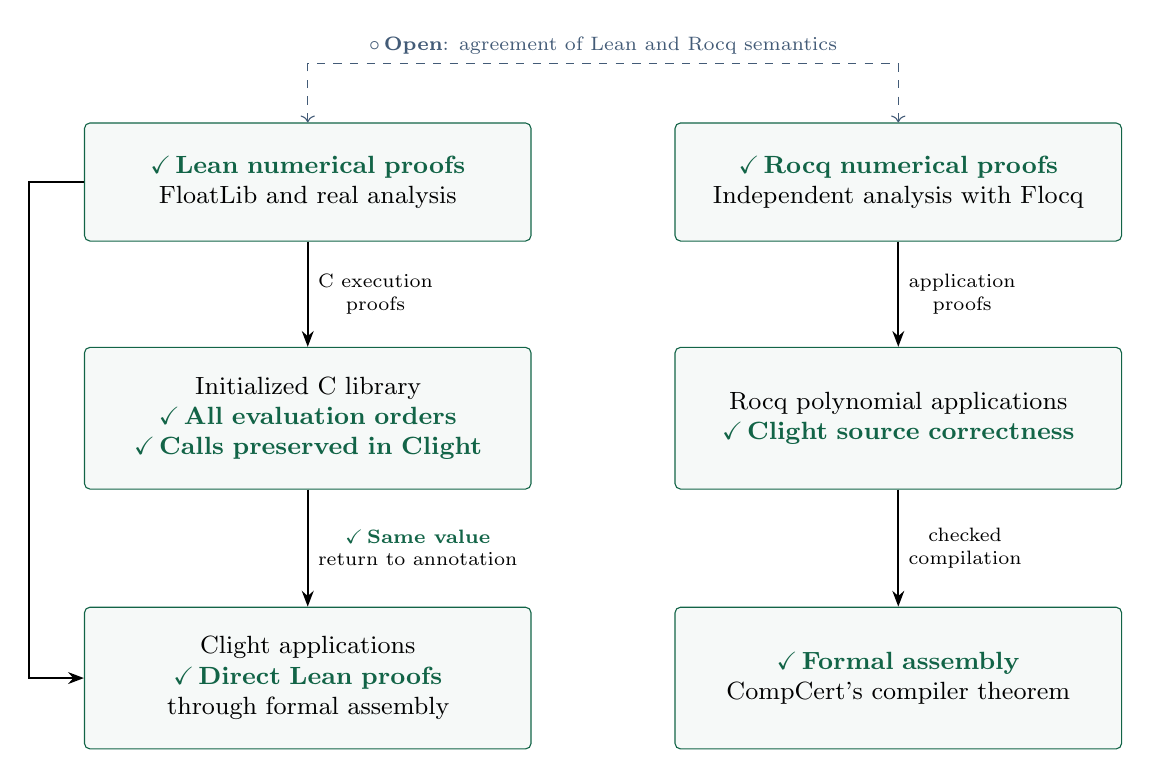
\begin{tikzpicture}[
 box/.style={draw=provedcolor,fill=provedcolor!4,rounded corners=2pt,
             align=center,text width=5.25cm,minimum height=1.5cm,
             font=\small,inner sep=6pt},
 arrow/.style={-{Stealth[length=2mm]},thick},
 note/.style={font=\scriptsize,align=center}]
 \node[box] (ln) at (0,0)
   {\checked{Lean numerical proofs}\\FloatLib and real analysis};
 \node[box] (rn) at (7.5,0)
   {\checked{Rocq numerical proofs}\\Independent analysis with Flocq};
 \node[box,minimum height=1.8cm] (lc) at (0,-3)
   {Initialized C library\\
    \checked{All evaluation orders}\\
    \checked{Calls preserved in Clight}};
 \node[box,minimum height=1.8cm] (rc) at (7.5,-3)
   {Rocq polynomial applications\\
    \checked{Clight source correctness}};
 \node[box,minimum height=1.8cm] (la) at (0,-6.3)
   {Clight applications\\
    \checked{Direct Lean proofs}\\through formal assembly};
 \node[box,minimum height=1.8cm] (ra) at (7.5,-6.3)
   {\checked{Formal assembly}\\
    CompCert's compiler theorem};
 \draw[arrow] (ln) -- node[right,note]{C execution\\proofs} (lc);
 \draw[arrow] (ln.west) -- ++(-0.7,0) |- (la.west);
 \draw[arrow] (rn) -- node[right,note]{application\\proofs} (rc);
 \draw[arrow] (rc) -- node[right,note]{checked\\compilation} (ra);
 \draw[arrow] (lc) --
   node[right,note]{\checked{Same value}\\return to annotation} (la);
 \draw[dashed,<->,opencolor] (ln.north) -- (0,1.5) --
   node[above,note]{\openproof{}: agreement of Lean and Rocq semantics}
   (7.5,1.5) -- (rn.north);
\end{tikzpicture}
\caption{The two developments within LeanQuadrature. Solid arrows connect
proved results; dashed arrows mark missing connections. Lean numerical
proofs support the initialized C library and applications checked through
assembly. The left vertical arrow compares the value returned by C with the value
reported by the application; it does not assert a general compilation
theorem. The right column describes our independent Rocq proofs. Both
columns end at formal assembly syntax, before native assembly and linking.}
\label{fig:boundaries}
\end{figure}

\subsection{Proving the compiled programs directly in Lean}

For the direct Lean proofs, we ran the ten
polynomial applications through CompCert and exported selected intermediate
programs: Cminor, CminorSel, the initial RTL and the RTL immediately before
register allocation, LTL, Linear, Mach, and formal x86-64 assembly.
Each exported program is a Lean term. For each intermediate language we
wrote the transition
rules and an executable checker over the same FloatLib-adapted value and
memory models used for Clight. We then proved, for each of the ten
programs at each stage, that execution from the initial state terminates
with the certified result annotation and exit status zero. Every reachable
state can finish, and no execution runs forever or gets stuck.

At formal assembly an order-$n$ run takes $153n+37$ semantic steps.
The Mach proofs check the generated return addresses against the translated
continuations at all sixteen call sites. We also relate selected parts of
adjacent stages, such as the contents and permissions of the global memory
blocks in Clight and Cminor.

The result is a proof of each imported program's behavior in the Lean
semantics. A general compiler theorem would have to relate the input and
output of every successful compilation. To reuse CompCert's theorem in
Lean, we would need to relate the exported syntax and adapted semantics to
their Rocq definitions, then justify interpreting the Rocq theorem in Lean.
Another approach would be a translation validator that checks each
compilation and has a proved soundness theorem.

\subsection{From a C return to an application result}

The library returns a binary64 value, while the application reports one
and exits. To relate them, let $R_n(v)$ mean that the initialized C
integrator, called with the polynomial callback and order $n$, returns $v$
with an empty trace. Let $A_n(t,s)$ mean that the corresponding initialized
assembly application terminates with trace $t$ and exit status $s$, and
write $T(v)$ for the single \code{quadrature-result} annotation carrying $v$.

\begin{theorem}[Agreement of C returns and assembly observations]
\label{thm:c-assembly-observations}
For every $1\le n\le10$, trace $t$, and exit status $s$,
\[
  A_n(t,s)
  \quad\Longleftrightarrow\quad
  \exists v,\; R_n(v)\ \land\ t=T(v)\ \land\ s=0.
\]
Both the C call and the assembly application terminate without getting
stuck. For the original two-point wrapper, the returned and reported value
has bits \code{0x3fead02c771c35ed} and integral error at most $0.00356$.
\end{theorem}

The proof compares each side with the same FloatLib result $F_n$.
The initialized C call can return only $F_n$, and the assembly application's
only final observation is $T(F_n)$ with status zero. The existing execution
proofs establish that both outcomes occur and that every execution
terminates. These statements hold for any external-call relation: the
library calls are internal, and the assembly execution uses only the
specified annotation.

A companion theorem relates returns from the actual normalized Clight
library to the authored Clight application's observations. Their cosine
bodies differ syntactically but evaluate the same rounded polynomial.
That theorem retains the Clight application proof's external-call
determinism premise. The direct C-to-assembly result above does not need
that premise.

This agreement supplies the result connection for these applications.
Their entry points were written in Clight, and the imported assembly trees
were checked directly. A proof that a compiler applied to the original C
text produces these trees would be a separate result, as would a theorem
relating the adapted Lean semantics to Rocq's.

\subsection{Using CompCert in Rocq}

The second route uses CompCert's theorem in Rocq. We reproved the numerical
results for the polynomial programs in
Rocq, independently of the Lean proofs, and composed them with compilation
and termination proofs. All ten orders have integral-error certificates
whose conclusions hold for every behavior of the compiled program.
Successful compilation is itself checked inside Rocq, so it does not remain
a hypothesis.

Evaluating CompCert inside the Rocq kernel needs a configuration that the
kernel can run. We supply executable definitions for the compiler's
external choices, disable selected optimizations and inlining, and use a
finite set of register-allocation candidates that CompCert's validator must
accept. The configuration also exposes computations needed by evaluation
and uses a bounded iteration procedure whose invariant theorem we reprove.
The certificate script rebuilds the compiler proofs from source. Its finite
allocator may fail on other programs, so the results describe this checked
compiler variant and these applications.

\subsection{Connecting the two proof systems}

The independent Rocq proofs supply the numerical premises for the
CompCert applications. Reusing the Lean proof would avoid repeating that
analysis. One route is a sound interpretation or translation of
the relevant arithmetic, program states, and propositions. Another is a
common certificate format with sound checkers in both systems. Either
approach must justify the interpretation of the checked result in the
receiving system.

Floating-point arithmetic shows what has to be related. The FloatLib and
Flocq models used here have different NaN policies, and paired certificates
show that unrestricted bitwise equivalence between them is false. For
quadrature the useful comparison concerns finite computations and must
preserve the sign of zero. We have proofs in both systems that
characterize rounding through integer quotients, remainders, parity, and
exponent alignment. Relating those integer representations is still open.

\subsection{From formal assembly to an executable}

The CompCert manual places assembly printing, assembling, and linking
outside the verified core. Our final property concerns a
\code{quadrature-result} semantic annotation and exit status zero in
formal assembly. The printer turns the annotation into a comment, so this
property does not yet describe a printed answer from a native executable.
Connecting it to one requires proofs about the intended output operation
and the remaining translation steps. CompCert could also compile C emitted
by Lean's own compiler. Its theorem would then cover the C compilation
step, and the Lean-to-C translation and runtime would still need
justification.

\section{Results}
\label{sec:evidence}

Table~\ref{tab:results} gives the results for the ten polynomial
applications. Each row identifies the binary64 answer and a proved bound on
its distance from $\sin1$. Lean and our Rocq development check these bounds
independently. At the higher orders the bounds are on the scale of rounding
and stored-table perturbations, and increasing the number of nodes does not
make these finite-precision bounds decrease at every step: the seven-node
bound is smaller than the eight-node bound.

\begin{table}[htbp]
\centering
\begin{tabular}{rlrl}
\toprule
\rowcolor{tablehead}
Nodes & Binary64 result bits & Error at most & Status\\
\midrule
1  & \code{3ff0000000000000} & $0.159$ & \proved{}\\
2  & \code{3fead02c771c35ed} & $0.00356$ & \proved{}\\
3  & \code{3feaed9520c8a014} & $3.1\cdot10^{-5}$ & \proved{}\\
4  & \code{3feaed5443a06327} & $1.5\cdot10^{-7}$ & \proved{}\\
5  & \code{3feaed548f3f6f46} & $4\cdot10^{-10}$ & \proved{}\\
6  & \code{3feaed548f08f234} & $8\cdot10^{-13}$ & \proved{}\\
7  & \code{3feaed548f090ce1} & $2\cdot10^{-15}$ & \proved{}\\
8  & \code{3feaed548f090cce} & $4\cdot10^{-15}$ & \proved{}\\
9  & \code{3feaed548f090ccf} & $4\cdot10^{-15}$ & \proved{}\\
10 & \code{3feaed548f090cd4} & $3\cdot10^{-15}$ & \proved{}\\
\bottomrule
\end{tabular}
\caption{Proved error bounds for the ten initialized polynomial applications.
The callback evaluates the degree-14 cosine polynomial with fixed rounding
at each operation.}
\label{tab:results}
\end{table}

LeanQuadrature~\cite{leanquadrature} contains the application proofs, the build
instructions, and a map from every result in this paper to its theorem
declaration. The full Lean build and transitive assumption checks cover the
project theorems, their private helpers, and the adapted CLean library, and
the only permitted axioms are \code{propext}, \code{Classical.choice}, and
\code{Quot.sound}. The Rocq compilation proofs have their own record of
assumptions, including the logical and external-semantics dependencies of
CompCert and Flocq. The project contains roughly 50,000 lines of Lean, a
large share of it imported program syntax, and about 10,000 lines of Rocq.
LeanPDE is a private dependency. The public source distribution does not
include it; readers who wish to reproduce the build should request access
from the author.

\section{Discussion}
\label{sec:conclusion}

The mathematical and numerical proofs draw heavily on existing Lean
libraries. mathlib provides the analysis needed for the general Gaussian
construction; LeanPDE contributes quadrature interfaces, concrete rules,
and certified symbolic calculation; FloatLib makes the binary64
computation executable inside the logic. LeanPDE contains the weighted
construction, remainder, convergence, and Legendre certificate proofs.
LeanQuadrature applies these results to certify the ten stored rules and
prove the programs that use them.
LeanPDE is essential to this implementation because we import those
definitions and theorems.
TorchLean is a transitive dependency of LeanPDE; we do not use its tensor
or neural-network interfaces.

The larger difference between the two systems appears in program
verification. Rocq supplies VST's C program logic and CompCert's compiler
theorem in the same proof system. Lean already has CLean's Clight contracts,
separation logic, function-pointer rules, and module-linking operations.
Our application proofs use its operational semantics directly.
Iris-Lean offers a further program-logic foundation, whose use here would
require a C/Clight language instance and verified rules for memory operations
and calls. The existing Lean infrastructure is substantial; the present
development does not establish VST's broader modular reasoning and automation,
or a transfer of CompCert's compiler theorem.

The source review gives concrete corrections to Appel and Bindel's
preliminary application argument. The two error bounds and three admitted helpers have
counterexamples; the remainder needs consistent indexing and a smoothness
premise; the table model must agree with the initialized C values.
The callback body proof and the incorrectly named Hughes specification
are separate program obligations. Our Lean proofs supply corrected
mathematical statements and verify the polynomial replacement. The public
derivative-bound work already moves toward stronger hypotheses, and the
missing quadrature VSU explains why the initializer and function-identifier
mismatches are not caught by the existing body proofs. These are unfinished
steps in the authors' development, not failures of VST's program logic.
The overflow
inequalities were transcribed into Lean and checked against the source by
inspection. The positivity counterexample was also checked against the
original statement in Rocq.

The C library's return values are now related to the application observations
through formal assembly. This is a result about the particular verified
programs, with an explicit change from a library return to a result annotation.
A general source-translation theorem would still have to justify parsing and
elaboration, including preprocessing and static-array handling, and a
compilation theorem would have to relate compiler inputs to outputs. Reusing
CompCert's compiler theorem in Lean adds a different obligation: proving a
sound interpretation of the Rocq semantics and results. A theorem about a
native executable's printed answer must also account for assembly
printing, assembling, linking, and the output operation.

\FloatBarrier
\appendix
\section{Gaussian quadrature in LeanPDE}
\label{sec:stewart-map}

LeanPDE supplies the Gaussian theory used here: weighted rules of every
positive order, orthogonal polynomials, roots, exactness, positive weights,
recurrence, remainder, and convergence. It also provides explicit Legendre
rules through four nodes and general root and weight certificates.

Table~\ref{tab:stewart} follows the 24 numbered paragraphs of Stewart's
\emph{Afternotes on Numerical Analysis}, Chapter 23, as used in Appel and
Bindel's Section 2~\cite{stewart}. The left column states the mathematical
step; the right names the LeanPDE result and explains its proof or scope.
Their PDF skips paragraph 14, whose root argument appears in the
\code{quadrature.v} comments.

For the compact-interval results, assume finite $a<b$, a continuous weight
$w>0$ on $[a,b]$, and $n>0$ nodes. Write $\I_w$ for the weighted integral,
$p_n$ for the degree-$n$ monic orthogonal polynomial, and $\ell_i$ for a
cardinal Lagrange polynomial. Stewart's indices $0,\ldots,m$ correspond to
$n=m+1$, so his derivative order $2m+2$ becomes $2n$ here.

LeanPDE also gives the sharp two-point estimate
\[
 \left|\int_a^b f(x)\,dx-Q_2(f)\right|
 \le \frac{M(b-a)^5}{4320},
 \qquad
 \left|f^{(4)}(x)\right|\le M,
\]
under $a<b$ and $f\in C^4([a,b])$. On $[-1,1]$ this is $M/135$.
The theorem is
\code{norm_integral_sub_gaussLegendreTwoRule_valueOn_le}
in LeanPDE's \code{GaussLegendrePeano} module. The general Hermite
remainder supplies the same coefficient and also gives a single point
witnessing the integrated remainder identity.
The companion
\href{https://github.com/Robertboy18/LeanQuadrature/blob/main/docs/stewart-comparison.md}{LeanPDE source map}
gives file links and precise hypotheses for the results below.

\begingroup
\small
\setlength{\tabcolsep}{4pt}
\renewcommand{\arraystretch}{1.13}
\begin{longtable}{@{}>{\raggedright\arraybackslash}p{0.45cm}
  >{\raggedright\arraybackslash}p{6.0cm}
  >{\raggedright\arraybackslash}p{8.75cm}@{}}
\caption{Stewart's Chapter 23, as followed in Appel and Bindel's
Section 2: the 24 mathematical steps and their current LeanPDE coverage.
The statements use $n$ nodes. Checkmarks mark available definitions
and proved results; alternative arguments and open cases are identified.}
\label{tab:stewart}\\
\toprule
\rowcolor{tablehead}
\P & Textbook statement or argument & LeanPDE result and proof\\
\midrule
\endfirsthead
\multicolumn{3}{@{}l}{\textit{Table~\ref{tab:stewart} continued:
Stewart's Chapter 23 and Appel--Bindel Section 2.}}\\
\addlinespace
\toprule
\rowcolor{tablehead}
\P & Textbook statement or argument & LeanPDE result and proof\\
\midrule
\endhead
\bottomrule
\endfoot
1 & Approximate the weighted integral $\I_w(f)$ by a sum of $n$ values,
$\Q_n(f)=\sum_i\lambda_i f(x_i)$. &
\checked{Defined}: \code{GaussianRule} and \code{GaussianRule.value}
represent and evaluate the rule. Its existence is proved using the
orthogonal polynomials and their roots below.\\
\addlinespace
2 & Keep the interval and weight fixed, and abbreviate integration
against $w$ by $\I_w$. &
\checked{Defined}: \code{polynomialIntegral} is the weighted integral
restricted to polynomials.\\
\addlinespace
3 & Integration commutes with addition and scalar multiplication
for integrable functions. &
\checked{Defined and proved}: \code{polynomialIntegral} is a linear map,
using mathlib's integral linearity.\\
\addlinespace
4 & Define orthogonality by $\I_w(pq)=0$, using the integral of the
product as an inner product. &
\proved{}: \code{momentInnerCore} constructs the polynomial inner product;
\code{polynomialIntegral_square_pos} proves positivity on nonzero squares.\\
\addlinespace
5 & Choose a monic polynomial $p_k$ of each degree $k$, with
$\I_w(p_i p_j)=0$ whenever $i\ne j$. &
\proved{}: \code{exists_monic_orthogonal} constructs the family by
orthogonal projection; \code{orthogonalPolynomial_unique} proves
uniqueness at each degree.\\
\addlinespace
6 & Every polynomial of degree at most $n$ has a unique expansion
in any monic family $p_0,\ldots,p_n$ with $\deg p_k=k$. &
The arbitrary-family expansion theorem is not separately formalized.
Orthogonal projection gives the family directly, so the Gaussian
construction does not need this intermediate result.\\
\addlinespace
7 & Prove that expansion by subtracting the leading multiple of
$p_n$, lowering the degree, and applying induction. &
\code{degree_sub_coeff_mul_lt} proves the degree reduction used in
the recurrence. It does not establish the full expansion and uniqueness
argument of paragraph 6.\\
\addlinespace
8 & An orthogonal polynomial $p_n$ is orthogonal to every polynomial
of degree below $n$. &
\proved{}: \code{orthogonalPolynomial_orthogonal}. This is a defining
property of the projection construction.\\
\addlinespace
9 & The family starts with $p_0=1$ and
$p_1(x)=x-\I_w(x)/\I_w(1)$, as determined by orthogonality to constants. &
\proved{}: \code{orthogonalPolynomial_zero} and \code{orthogonalPolynomial_one},
including the weighted mean in the degree-one coefficient.\\
\addlinespace
10 & Inner products determine the coefficients of $p_n$ and $p_{n-1}$
when expressing $xp_n-p_{n+1}$ in the orthogonal family. &
\proved{}: \code{recurrenceAlpha} and \code{recurrenceBeta} give those
ratios of integrals; the recurrence theorem proves the identity.\\
\addlinespace
11 & All earlier terms vanish: $xp_j$ has degree below $n$ when
$j<n-1$, so it is orthogonal to $p_n$. &
\proved{}: lower-degree orthogonality removes these terms in the proof
of the three-term identity. No separate infinite coefficient list is needed.\\
\addlinespace
12 & After the first two polynomials, each $p_{n+1}$ is obtained
from $xp_n$, $p_n$, and $p_{n-1}$ by a three-term recurrence. &
\proved{}: \code{orthogonalPolynomial_recurrence}, with
\code{recurrenceBeta_eq_norm_ratio} and \code{recurrenceBeta_pos}.
The recurrence is derived after the projection construction.\\
\addlinespace
13 & The degree-$n$ orthogonal polynomial has exactly $n$ real,
distinct roots, all inside $(a,b)$. &
\proved{}: \code{orthogonal_splits}, \code{orthogonal_squarefree}, and
\code{orthogonal_root_mem_Ioo} give splitting, simplicity, and interiority.\\
\addlinespace
14 & Multiply $p_n$ by the product of the linear factors at its
sign-changing roots. Too few such roots would make orthogonality
contradict a nonzero integral. &
\checked{Alternative proof}: \code{orthogonal_factor_has_root} forces
each nonconstant factor to have an interval root. Factorization gives
splitting; separate positivity arguments give simplicity and exclude endpoints.\\
\addlinespace
15 & Use the roots as nodes and set $\lambda_i=\I_w(\ell_i)$.
Lagrange interpolation then gives exactness below degree $n$. &
\proved{}: \code{interpolatoryWeight} and \code{interpolatory_exact};
\code{GaussianRule.weights_eq_interpolatoryWeight} identifies the
Gaussian weights with these integrals.\\
\addlinespace
16 & For $\deg f\le 2n-1$, divide $f=p_nq+r$ with
$\deg q,\deg r<n$. Orthogonality and interpolation give $\Q_n(f)=\I_w(f)$. &
\proved{}: \code{gaussian_exact} follows this division argument.
The $p_nq$ term vanishes at the nodes and has zero weighted integral;
the rule integrates $r$ exactly.\\
\addlinespace
17 & Apply exactness to $\ell_i^2$. Its quadrature value is
$\lambda_i$, and its weighted integral is positive. &
\proved{}: \code{gaussian_weight_pos} uses this squared-Lagrange
argument to prove every weight positive.\\
\addlinespace
18 & The weights sum to $\I_w(1)$. The quoted prose also concludes that
each weight is at most one. &
\proved{}: \code{sum_weights} and \code{weight_le_mass}.
The general bound is $\lambda_i\le\I_w(1)$.
The Rocq theorem already states this mass bound; the bound one follows
under unit-mass normalization.\\
\addlinespace
19 & For sufficiently smooth $f$, the quadrature error is
$\I_w(p_n^2)$ times $f^{(2n)}(\xi)/(2n)!$ at some interval point $\xi$. &
\proved{}: \code{hermite_remainder}, \code{GaussianRule.remainder},
and \code{GaussianRule.abs_error_le}. Hermite interpolation gives the
pointwise error; the integrated identity uses the continuity assumptions
in Section~\ref{sec:mathematics}.\\
\addlinespace
20 & Approximate a continuous function uniformly by polynomials.
Positivity and increasing exactness then give $\Q_n(f)\to\I_w(f)$. &
\proved{}: \code{gaussian_rules_converge} follows this uniform-approximation
argument on a compact interval with fixed positive continuous weight.\\
\addlinespace
21 & Choose $w=1$ on $[-1,1]$. The resulting family consists of
the monic Legendre polynomials and yields Gauss--Legendre quadrature. &
\proved{}: the general construction specializes to unit weight.
Explicit rules through four nodes are identified with the monic Legendre
family. General root and weight certificates support the stored tables.\\
\addlinespace
22 & Gauss--Laguerre quadrature treats an integral on $[0,\infty)$. &
\openproof{}: the corresponding unbounded-interval construction,
remainder, and convergence theory are outside this development.\\
\addlinespace
23 & Gauss--Hermite quadrature treats an integral on the whole real line. &
\openproof{}: this unbounded-interval quadrature theory is outside the
development. Hermite interpolation in paragraph 19 is a different result.\\
\addlinespace
24 & Other choices of interval and weight produce Gaussian rules
suited to other integrals. &
\code{exists_gaussian_quadrature} applies to any positive continuous
weight on a compact interval. Individual named families require their own
specialization and certificates.\\
\end{longtable}
\endgroup

\begingroup
\small
\bibliographystyle{plain}
\bibliography{references}
\endgroup

\end{document}
